\capitulo{2}{Objetivos del proyecto}

A continuación se detallan los objetivos que se han llevado a cabo en este proyecto. Se han dividido
en tres secciones, la primera trata de los objetivos generales (qué se ha querido implementar), en
la segunda se tratan los objetivos técnicos (qué herramientas se han usado) y por último se abordan
los objetivos personales (por qué se escogió este proyecto).

\section{Objetivos generales}

En este Trabajo de Fin de Máster se persigue dotar a las rutas que una persona puede seguir en sus días de vacaciones de un significado semántico. Es decir, se pretende asignar una palabra clave a posiciones significativas dentro de la ruta que dicha persona ha seguido o está siguiendo en un momento determinado. Enfocándose en una visita turística, estas palabras clave estarán relacionadas con lugares turísticos de la localidad visitada, por ejemplo, su plaza mayor, su catedral o sus iglesias, sus museos o edificios de interés, etc. No obstante, se tienen en cuenta otros lugares como pueden ser centros comerciales, bancos, o restaurantes. Estos puntos o zonas reciben el nombre de Puntos de de Interés (PDI o POI, por sus siglas en inglés).

\subsection{PDI (Point de Interest}
Como se ha descrito anteriormente, un Punto de Interés (PDI) es un lugar especificado mediante coordenadas geográficas que es interesante o útil para un gran número de personas. Este término es usado de forma general en aplicaciones software de cartografía o navegadores GPS.

Un PDI constará, como mínimo, de latitud y longitud pero también se suele incluir cierta información como un nombre, su descripción, la altitud o un número de teléfono. Cada PDI puede llevar asociado un cierto icono representativo usado por las aplicaciones para dotar de una mayor facilidad de uso al usuario. La Figura \ref{puntosdeinteres} muestra un ejemplo de estos PDI sobre un mapa de Open Street Maps. En este caso, estos puntos marcan un hospital, un parking, un taller de automóviles, diversas paradas de autobús, bancos e, incluso, semáforos.

\begin{figure}[h]
  \centering
    
\includegraphics[width=0.6\textwidth]{../img/poi/poi.png}
  \caption{Puntos de Interés señalados en el mapa}
  \label{puntosdeinteres}
\end{figure}


Una vez se conocen los PDI por los que una persona ha pasado, se pueden reconocer los más significativos y asignar a su ruta. En este momento se puede decir que la trayectoria seguida es una trayectoria semántica. De esta forma se pasará de una serie de coordenadas (latitud, longitud) a un recorrido cíclico como el de la Figura \ref{rutasemantica}. En este recorrido se observa la salida desde el Hotel Zola, pasando por lugares de interés como la Torre Eiffel, el Palacio Borbón o el Museo del Louvre, terminando en el Restaurante \textit{Babylone} antes de regresar al punto de origen.

\begin{figure}[h]
  \centering
    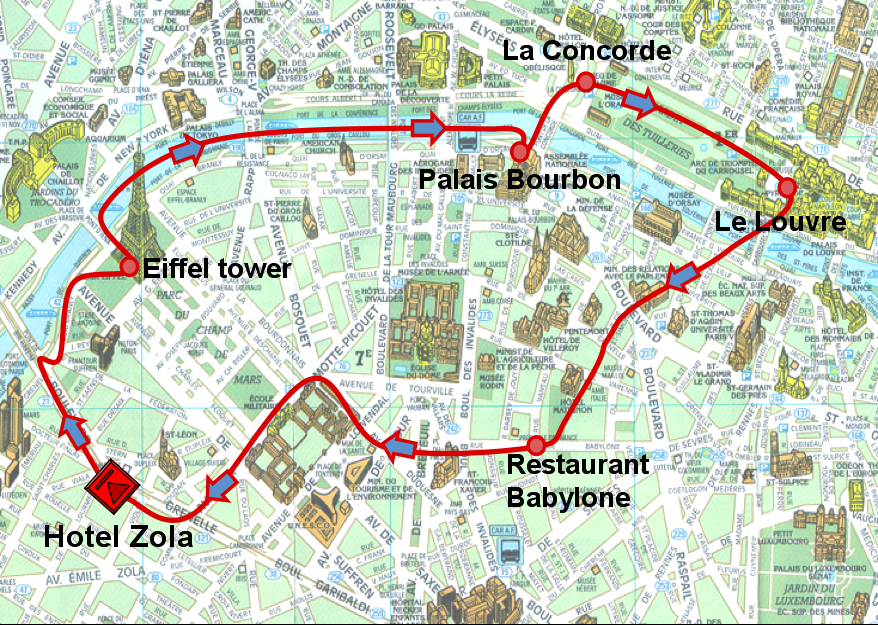
\includegraphics[width=0.6\textwidth]{../img/poi/ruta.png}
  \caption{Ruta semántica sobre París}
  \label{rutasemantica}
\end{figure}


Siguiendo la filosofía de Open Street Maps, se pueden distinguir los PDI situados sobre una zona concreta dependiendo del tipo o del lugar al que hacen referencia. Dentro de estos mapas, estas categorías son denominadas ``Amenities''.

\subsection{Trayectoria semántica}

La consecución de distintos PDI sobre una misma ruta, define una trayectoria semántica. Esta trayectoria semántica puede estar formada por los puntos mencionados anteriormente, sobre el mapa del centro de París.

\subsection{Análisis de trayectorias semánticas}

El interés de una trayectoria semántica radica en los tipos de Puntos de Interés visitados por una persona que puede ser considerada turista en una localidad. De esta forma se puede categorizar cada ruta por los sitios de interés visitados. A continuación se muestra un ejemplo sencillo.

Una persona que realiza una visita turística en una ciudad puede estar interesada en visitar su catedral, sus iglesias o monasterios más importantes, etc. Englobando todo tipo de edificios destinados al culto religioso. Sin embargo, otra persona puede realizar una visita a los museos o monumentos de arte moderno combinándola con restaurantes de ``autor''. Cada persona puede que tenga un ritmo diferente y sus visitas se duren un periodo de tiempo diferente.

En estos dos casos, es evidente, que ambas personas buscan lugares de interés turístico completamente diferentes. Seguramente estos patrones se repitan en las distintas visitas turísticas que realicen a otras localidades del país o, incluso, de otros países.

Habiendo realizado un análisis de las rutas o trayectorias que cada persona sigue, es posible recomendar a dicha persona una ruta adecuada en una ciudad que no haya visitado. De esta forma se ahorrará un tiempo valioso durante la preparación del viaje, que podrá ser aprovechado en la visita de los lugares seleccionados.


\section{Objetivos técnicos}

A la hora de implementar los objetivos marcados en este Trabajo de Fin de Máster, se han debido resolver distintas cuestiones técnicas. En esta sección se tratarán estos objetivos.

\subsection{PostGIS}

PostGIS es una extensión espacial para las bases de datos relacionales PostgreSQL. Añade soporte  para objetos geográficos permitiendo realizar consultas espaciales en SQL.

Este soporte se encuentra respaldado mediante tres características únicas de esta extensión: tipos de datos espaciales, índices espaciales y funciones que actúan sobre ellos. Esta información espacial será almacenada en una columna de tipo ``GEOMETRY''.

Cabe destacar que PostGIS ha sido certificado por el Open Geospatial Consortium (OGC) garantizando la interoperabilidad con otros sistemas.


\subsection{PostgreSQL}
Viendo la dependencia que PostGIS tiene sobre PostgreSQL, ha sido necesario el uso de este Sistema Gestor de Base de Datos para dar soporte a la extensión comentada. El uso de este SGBD no entraña una complicación superior o diferente a la del uso de cualquier otro sistema.


\subsection{QGIS}
QGIS es un Sistema de Información Geográfica de código libre. Permite manejar distintos tipos de objetos mediante las bibliotecas GDAL y OGR además de comunicarse con Bases de Datos. La interfaz de QGIS permite visualizar mapas de Open Street Maps, situar rutas sobre dichos mapas, consultar rutas a PostGIS, descargar ficheros de  extensión OSM. Estos ficheros contienen todo tipo de información sobre una sección determinada de un mapa. Por ejemplo, se puede extraer todo tipo de información de las calles de una ciudad concreta, sobre sus POI, etc. 

\subsection{Biblioteca ``tSemanticas''}
La biblioteca que acompaña a este trabajo ha sido desarrollada en Java.

\section{Objetivos personales}

El presente Trabajo de Fin de Máster ha supuesto un reto personal puesto que en el momento de comenzar el mismo no se contaba con los conocimientos suficientes como para llevarlo a cabo. Durante los meses en los que se ha trabajado sobre este documento, se ha realizado un esfuerzo por aprender las tecnologías necesarias así como todos los conceptos teóricos asociados a las mismas.

